\section{Monte Carlo Variance Reduction}
\label{sec:MCvar}

Monte Carlo methods for radiation transport are used in the nuclear
engineering community for a wide spectrum of application problems. Without any
variance reduction techniques, Monte Carlo methods aim to emulate
the transport of a particle from birth, through physical interaction, to death
by randomly sampling probabilities of the physics the particle could encounter, e.g.\ production, elastic and inelastic
scattering, absorption, etc.
This process of transporting a single particle
is repeated millions of times, which is analogous to transporting
millions of particles throughout the problem. When the user achieves a
sufficient
number of samples to reach the desired statistical precision for
the region of interest, the
simulation will be complete. 

However, this approach of simulating each
particle, no matter whether it is likely to contribute to the tallied result,
can be extraordinarily computationally inefficient depending on the problem. A
user could waste time simulating millions of unusable particles and still not
reach the desired statistical precision for the tally. Variance
reduction techniques were developed to address this issue. In general, these
techniques cause the Monte Carlo transport to more effectively
contribute to a particular result, while not biasing the result.

\subsection{Statistical Background}
\label{subsec:StatBkgnd}

Variance reduction techniques are rooted in statistics, so we will begin our
discussion of variance reduction techniques with a brief primer on the
statistical background relevant to Monte Carlo radiation transport. Sections
\ref{subsubsec:PopStat} through \ref{subsubsec:FOM} are summarized from
\cite{lewis_computational_1984} and \cite{mcnp_manual_v1}.
Monte Carlo
methods transport many randomly sampled
particles, and when those particles reach a region of interest, they are scored
in a tally. The statistical precision of the tally
will reflect the total number of particles that were sampled in or at this
region or surface.
The reliability of the answer obtained in this region depends
on the quantity of these particles.
%and the amount of time taken to move the particles on
%their respective random walks through space to the region.
% RNS: Why would the statistics depend on time?

\subsubsection{Population Statistics}
\label{subsubsec:PopStat}

In radiation transport, one desires to estimate some response in phase-space.
This response is the average behavior of the physical interactions in some
differential phase-space in energy, space, or time. If the probability density
function, $f(x)$, for the response is known exactly,
then the response in $dx$ can be calculated exactly by the true
mean, or
\begin{equation}
  \bar{x} = \int_{-\infty}^{\infty} xf(x) dx .
\end{equation}
Rarely is $f(x)$ known
exactly, so instead it is sampled.
Using $N$ randomly sampled particles, the estimate of the true mean value is given as
\begin{equation}
  \hat{x} = \frac{\sum_{i=1}^{N}{x_i}}{N} ,
\end{equation}
where $x_i$ is the i$^{th}$ event. $\hat{x}$ is the sample mean, or the
estimated value of $\bar{x}$
based on the $N$ number of samples that were used to calculate $\hat{x}$. As $N
\rightarrow \infty$, $\hat{x}$ will $\rightarrow \bar{x}$, which is given by the
Strong Law of Large Numbers \cite{mcnp_manual_v1}.
$\hat{x}$ in itself is a useful measure, but determining the spread of values
about $\hat{x}$ is also an important measure. This is called the variance. The
true variance of the distribution is
\begin{equation}
  \sigma^{2}\big( x \big) = \bar{x^2} - \bar{x}^2 ,
\end{equation}
and the standard deviation is the square root of the variance
\begin{equation}
  \sigma\big(x \big) = \big( \bar{x^2} - \bar{x}^2 \big)^{1/2}.
\end{equation}
The variance of the sampled distribution differs, as a finite number of samples
are used to calculate $\bar{x}$ and $\sigma$. The sample variance is defined by:
\begin{equation}
S^{ 2 }=\sum _{ i=1 }^{ N }{ \frac { (x_{ i }-\hat { x } )^{ 2 } }{ N-1 }  }
             \cong \widehat{x^2}-\hat{x}^2 ,
\label{eq:Var}
\end{equation}
where
\begin{equation}
  \widehat{x^2} = \frac{1}{N}\sum_{i=1}^{N} x_i^2 ,
\end{equation}
and the sample standard deviation is given by
\begin{equation}
  S = \big( \widehat{x^2}-\hat{x}^2 \big)^{(1/2)} .
\end{equation}

For Eqn. \eqref{eq:Var} to hold true, the number of samples must be large.
$S^2$ is the sample estimate of the true variance, $\sigma^2$. %The variance
%tells the observer how spread the sampled values are about the mean.
% RNS: already stated
The variance of the estimate of the mean value about $\bar{x}$ is:
\begin{equation}
S^{ 2 }_{ \hat { x }  }=\frac{S^2}{N}.
\label{eq:VarMean}
\end{equation}
From \eqref{eq:VarMean}, one can see the relationship between the sample standard
deviation and the standard error of $\hat{x}$ about $\bar{x}$ is
\begin{equation}
S_{ \hat { x }  }=\sqrt { \frac { S^{ 2 } }{ N }  } =\frac { S }{ \sqrt { N }}.
\label{eq:VarN}
\end{equation}
$S_{\hat{x}}$ is the standard error of the estimate of the sample mean.
The relative error normalizes the standard error by estimate of the mean
\begin{equation}
R = \frac{S_{ \hat { x }  }}{\hat{x}} .
\label{eq:RelativeErr}
\end{equation}
As a result, $S$, $R$, and $N$ follow the relationship
\begin{equation}
S^2\:\propto\: R^2\:\propto\:\frac{1}{N} .
\label{eq:S to R}
\end{equation}

\subsubsection{The Central Limit Theorem}
\label{subsubsec:CLT}

Suppose that $\hat{x}$ is calculated from several independent random particles
to estimate $\bar{x}$. At what point does one conclude that $\hat{x}$ sufficiently
reflects $\bar{x}$?
The central limit theorem (CLT) \cite{lewis_computational_1984, mcnp_manual_v1}
is a very powerful supplement to the quantities
described in Section \ref{subsubsec:PopStat}. The CLT states that for large N,
$\hat{x}$ will have a limiting distribution $f_N(\hat{x})$, and that distribution will be a
normal distribution
\begin{equation}
  f_N\big(\hat{x}\big) \approx \frac{1}{\sqrt{2\pi} \sigma(\hat{x})}\
           \exp\Bigg[ \frac{-\big( \hat{x}- \bar{x}\big)^2}{2\sigma^2(\hat{x})} \Bigg],\
           \quad N \rightarrow \infty.
  \label{eq:CLT1}
\end{equation}
The standard deviation of $\hat{x}$ can be related to the standard deviation of
the samples by
\begin{equation}
  \sigma(\hat{x}) = \frac{\sigma(x)}{\sqrt{N}}.
\end{equation}
Replacing this in Eq. \eqref{eq:CLT1} give
\begin{equation}
  f_N\big(\hat{x}\big) \approx \sqrt{\frac{N}{2*\pi}} \frac{1}{\sigma(x)}\
           \exp\Bigg[ \frac{-N\big( \hat{x}- \bar{x}\big)^2}{2\sigma^2(x)} \Bigg],\
           \quad N \rightarrow \infty
  \label{eq:CLT2}
\end{equation}
and allows us to use known values for $\hat{x}$ and an approximation of $\sigma(x)$
using $S$ to determine the probability density function of the sample means
$f_N(\hat{x})$. 
%RNS: I'm a little confused. Maybe some additional punctuation is needed? 
Because $f_N(\hat{x})$ is normally distributed, we can find the
probability that $\hat{x}$ lies in $\bar{x} \pm \epsilon$ with
\begin{equation}
  P\big\{\bar{x} - \varepsilon < \hat{x} \leq \bar{x} + \varepsilon\big\} = \
   \int_{\bar{x}-\varepsilon}^{\bar{x}+\varepsilon}f_N\big( \hat{x} \big) d\hat{x}.
   \label{eq:probmean}
\end{equation}
Placing our definition for the distribution of $\hat{x}$, which is $f_N(\hat{x})$, into Eq.
\eqref{eq:probmean}, changing the limits of integration, and changing the
variables such that $t = \sqrt{N/2}*(\hat{x}-\bar{x})/\sigma(x)$, this becomes
\begin{equation}
  P\big\{\bar{x} - \varepsilon < \hat{x} \leq \bar{x} + \varepsilon\big\} = \
  \frac{2}{\sqrt{\pi}} \int_0^{(\sqrt{N/2})(\varepsilon/\sigma(x))} e^{-t^2} dt\:.
\end{equation}
Recalling the definition of the error function, we obtain
\begin{equation}
  P\big\{\bar{x} - \varepsilon < \hat{x} \leq \bar{x} + \varepsilon\big\} = \
    \erf\Big[\sqrt{\frac{N}{2}} \frac{\varepsilon}{\sigma(x)}\Big].
\end{equation}
Then, using the calculated estimation for $\sigma(x)$ and $S$, and using Eq.
\eqref{eq:VarN}, the error function reduces to be
a function of $\varepsilon$ and $S_{\hat{x}}$ only
\begin{equation}
    \erf\Big[\sqrt{\frac{N}{2}} \frac{\varepsilon}{\sigma(x)}\Big] = \
    \erf\Big[\sqrt{\frac{1}{2}} \frac{\varepsilon}{S_{\hat{x}}}\Big] .
\end{equation}
Should $\varepsilon$ be chosen to be a function of $S_{\hat{x}}$, the error
function reduces further and becomes merely an evaluation as multiples (M), of
$S_{\hat{x}}$ and $\sqrt{1/2}$. For the first few multiples of the standard
error, this is evaluated as
\begin{equation}
  P\big\{\bar{x} - M S_{\hat{x}} < \hat{x} \leq \bar{x} + M S_{\hat{x}} \big\} =
  \begin{cases}
    .683, & M = 1, \\
    .954, & M = 2, \\
    .997, & M = 3
  \end{cases}  .
\end{equation}

The central limit theorem tells us that the sample mean follows a normal
distribution, regardless of the distribution of the underlying sample, as the
number of samples approaches infinity. This
means that no matter what distribution is being sampled, the sampled mean will
have this expected behavior. As a result, given a calculated value for
$\hat{x}$ and $S$, the probability that $\hat{x}$ is near $\bar{x}$ is known
and calculable.
Further, the central limit theorem shows that this distribution is approached
very quickly as N increases, with most problems only requiring $N > 30$
\cite{lewis_computational_1984}. Note
that N is not the total number of samples, but the number of samples required to
calculate each mean.

However, for the central limit theorem to hold, a number of
requirements must be satisfied. Ss with all of the quantities in Section
\ref{subsubsec:PopStat},
% RNS: what is this frist clause?
 each $x_i$ is assumed to be randomly sampled from the same distribution as all $x_i$s and
independent of every other $x_i$. If some region of phase space is omitted
accidentally, these values will not be reflective of the true $f(x)$, and so
$\hat{x}$ will not approximate $\bar{x}$. Further, for $S$ to be a
good approximation of $\sigma(x)$, a large number of samples must contribute
to the calculation of $\hat{x}$. Further, the central limit theorem assumes that
$f(x)$ is a probability density function that can be sampled and has a variance
that exists. As a result, one must be reasonably sure that all of these
requirements are satisfied if using Monte Carlo sampling methods.

\subsubsection{The Figure of Merit}
\label{subsubsec:FOM}

The equations in the preceding sections describe how to estimate the statistics
of a population given a finite number of samples. In radiation transport, a
user seeks to estimate some response, the relative error associated with that
response solution, and the time it takes to obtain those values. Equation
\eqref{eq:S to R} described the relationship between the sample variance, the
relative error, and the number of particles as
\begin{equation*}
S^2\:\propto\: R^2\:\propto\:\frac{1}{N} .
\end{equation*}
The relationship between the relative error, $R$, and the number of particles, $N$,
%\begin{equation*}
%  R^2\:\propto\:\frac{1}{N}
%\end{equation*}
will be some constant value:
\begin{equation*}
 C_1 = R^2N .
\end{equation*}

As a problem is simulated, the number of particles run, $N$, will increase
proportionally to the computational transport time, $T$. Therefore, the
relationship between $R$ and $T$ should also be a constant.
\begin{equation*}
  C_2 = R^2T
\end{equation*}

The figure of merit (FOM) shown in Eqn.\ \eqref{eq:FOM}
is the most commonly reported metric using this relationship that is reported.
It is widely used in quantifying the effects of variance reduction methods.
Because it uses the inverse quantity of the relative error and time, a
``good'' result would be obtained from a low relative error in a short amount of
time, resulting in a high numerical value FOM.
\begin{equation}
FOM=\frac { 1 }{ R^{ 2 }T }
\label{eq:FOM}
\end{equation}
Further, a user may desire to determine how long a problem must be run to obtain
a desired relative error. In that case, Eqn.\ \eqref{eq:FOM} can simply be
rearranged to
\begin{equation*}
  R = \frac{1}{(FOM*T)^{1/2}} .
\end{equation*}

The figure of merit is a very useful tool, but it still is limited by statistical
precision in calculating $R$.
It is worth noting that early on in a transport simulation,
when too few particles have been simulated to
effectively capture $S$ or $\hat{x}$, the FOM will oscillate.
Eventually, the FOM will converge to a relatively constant value. This behavior can
also be used to determine whether one has sufficiently sampled the
region in which they are quantifying the response.

\subsection{Variance Reduction Methods for Monte Carlo Radiation Transport}
\label{subsec:MCVR}
MCNP \cite{hendricks_mcnp_1985, brown_mcnp_2002, mcnp_manual_v1}
has a number of techniques for variance
reduction that are accessible to users. These variance reduction
techniques fall
into four general categories: truncation methods, population control methods, modified
sampling methods, and partially-deterministic methods. Of importance for this
project are
population control methods and modified sampling methods, which are discussed in
a number
of the papers referenced herein. Truncation methods and partially-deterministic
methods do not contribute to and are not the focus of this work,
so will only be touched upon briefly. Note that while this
discussion will tend to focus towards the variance reduction methods in MCNP,
these
methods are by no means limited to this single software package. %A
%number of other Monte Carlo radiation transport packages also include these
%methods. RNS: not needed

% RNS: May want to either create another layer of subsection or bold the names of the vr straregies to help them stand out / be delineated. 
Population control methods adjust the particle population in the problem to
obtain better sampling in regions of interest by preferentially increasing or
decreasing the particle population.
The first two types of population control methods that will be discussed
are called splitting and rouletting.
Splitting is a method by which the particle population can be increased by
splitting a single higher-weight particle into several lower-weight particles.
Rouletting, conversely, reduces the particle population by stochastically
killing particles. Particles that survive a rouletting routine have their weight
adjusted higher, thereby conserving weight in the routine.
Both splitting and rouletting maintain a
fair game by adjusting the particle weights; the sum of the child particle weights is the same as the parent
weight as it entered the routine. 
%RNS: I think this is only on statistical average. Always true for splitting, statistically true for rouletting, right?

To use population control methods effectively as variance reduction techniques,
splitting is performed in high-importance regions to increase the particle
count, and thus the sampling, in important regions. Conversely, rouletting is
performed in
 low-importance
  regions to reduce the particle population in regions that are unimportant to
  the tally result.
Splitting and rouletting can be applied to include geometry, energy and time,
  as well as a weight cutoff.
  % RNS: weight cutoff is a truncation method...

Rouletting and splitting are often implemented through ``weight window"s. 
% RNS: I wouldn't talk about it that way. Rouletting and splitting are still separate algorithms. 
Figure \ref{fig:ww-mcnp}
illustrates the weight window concept.
%
\begin{figure}
  \centering
  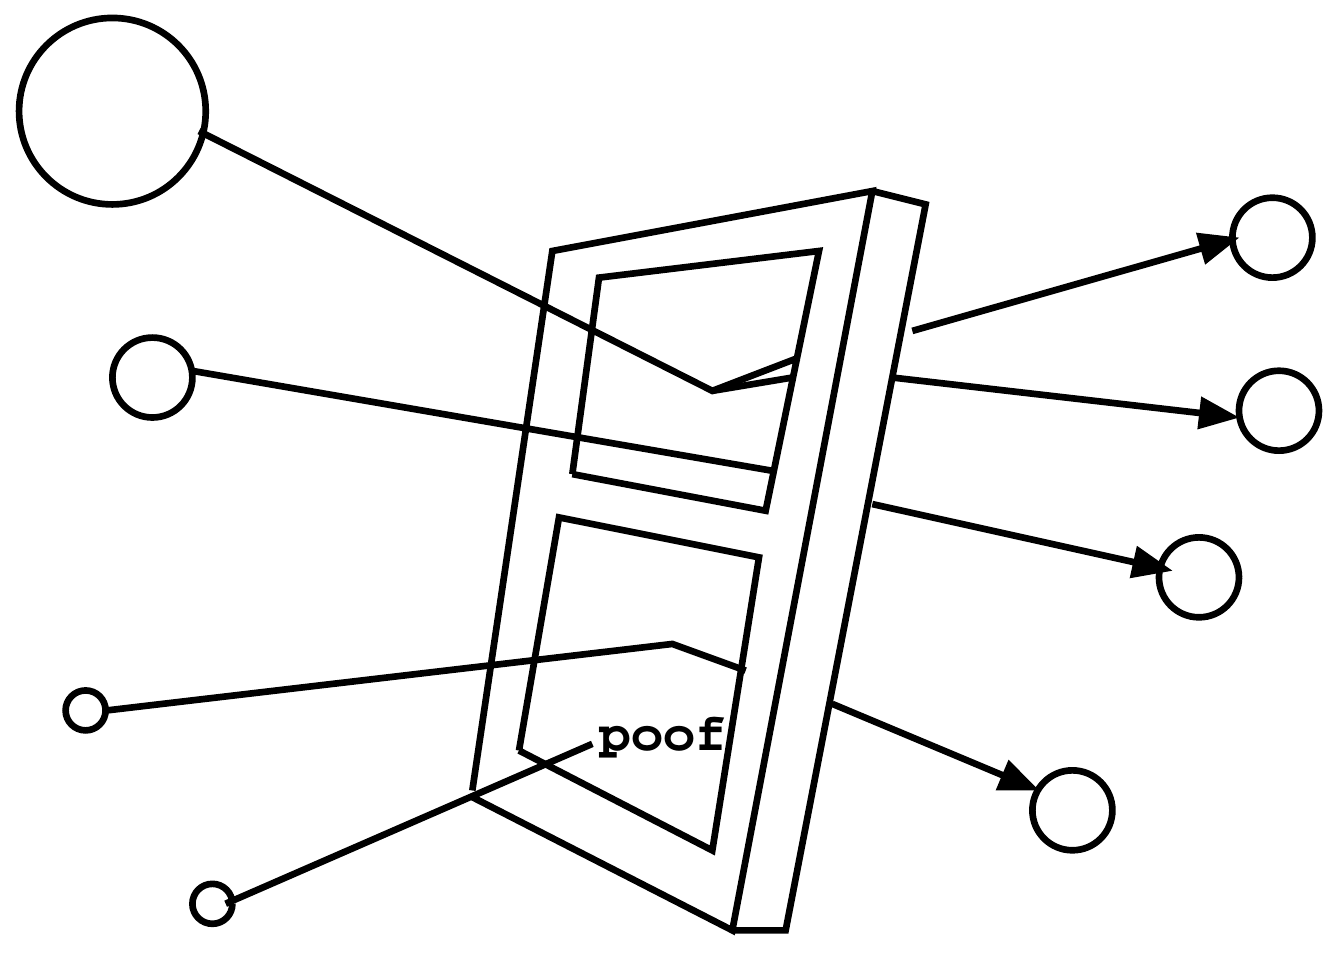
\includegraphics[width=0.5\textwidth]{./chapters/lit_review/figures/ww-mcnp.png}
  \caption[Weight window illustration]{Cartoon illustration of a weight window,
    adapted from \cite{brown_mcnp_2002, mcnp_manual_v2}}
  \label{fig:ww-mcnp}
\end{figure}
%
The top particle entering the weight window is a single, high-weight
particle. The weight of this particle is above the weight window bounds, so as
it enters the weight window it is split into multiple particles whose weight is
within the window bounds. The second particle entering the window is within the
weight window bounds, so it retains its weight and is not split or rouletted.
The last two particles entering the window have weights lower than the bound.
They undergo a rouletting routine and one particle is killed and the surviving
particle is increased in weight. As these particles leave the window, all of
them have weights within the range of the window. This will reduce the variance
of the particles contributing to a tally in that region. 

However, the user is
faced with estimating or calculating a significant number of parameters to
determine weight windows for the entire problem. In the best case with an
experienced user, this may just take time. With an inexperienced user or a
difficult problem this may be too difficult to do without some automated
assistance.

% RNS: I'd note in here somewhere that angle can also be included--there's no reason that it can't be done. It just isn't in practice. 
It should be noted that
while splitting and rouletting can be performed on a single variable--energy,
space, or time--the weight window is either energy-space
dependent or space-time dependent. Further, the weight window will split or
roulette depending on the particle weight entering the window. Splitting and
rouletting on their own either increase or decrease the particle weight
proportional to $I'/I$ no matter what the entering particle weight is. 
% RNS: need to define I and I'
As a
result, poorly chosen splitting or rouletting parameters can still
result in tallies with significant variance because particle weights may still span a wide
range.

Modified sampling methods adjust transport by sampling from a different probability
distribution function than the actual distribution for the problem. This is
possible if, as with population control methods, the particle weights are adjusted
 accordingly.
 The new probability distribution function should bias particles in regions of high
 importance to the problem tallies. In MCNP, a number of modified sampling
 methods exist.
 These include the exponential transform, implicit capture, forced collisions, source
 biasing, and neutron-induced photon production biasing.

The exponential transform modifies particle transport from the analog problem by
artificially modifying the macroscopic cross section, and thus the
distrance-to-collision, to move particles in important directions. In directions
of higher importance, the cross section is reduced, and particles can flow more
freely. In directions of lower importance, the cross section is increased, and
particles more frequently interact, thereby increasing their probability of
directional change or absorption. The transformed cross section used by the
exponential transform is defined by
%
\begin{equation}
  \Sigma_t^* = \Sigma_t(1-p\mu) ,
  \label{eq:ExTrns}
\end{equation}
%
where $\Sigma_t^*$ is the transformed total cross section, $\Sigma_t$ is the
true total cross section, $p$ is the transform parameter, and $\mu$ is the
cosine of the angle between the preferred direction and the particle's transport
direction \cite{mcnp_manual_v1, mcnp_manual_v2, hendricks_mcnp_1985}.

Because the particle's transport is adjusted in the exponential transform, the
particle weight must be adjusted accordingly. This is given by
%
\begin{equation*}
  \begin{split}
  w^* &= \frac{\Sigma_t e^{-\Sigma_t s}}{\Sigma_t^* e^{-\Sigma_t^* s}} \\
      &= \frac{e^{-\rho \Sigma_t \mu s}}{1-p\mu}, \\
  \end{split}
  \label{eq:ExTrnsWt}
\end{equation*}
%
where $s$ is the phase space of particle residence. This weight adjustment
ensures that the particle weight is conserved throughout transport, even as
the cross section is altered. Because the cross section in the problem is both
energy and material dependent (depending on the geometry), the exponential
transform will be dependent on space and energy, and particles will be biased in
both. While a powerful method, the exponential transform is quite difficult to
use and if $p$ is chosen poorly this method can perform quite poorly. Further,
the user has to know quite a bit about the problem physics and material to choose an
optimal quantity for $p$.

Source biasing, rather than preferentially adjusting particles' directionality
by way of adjusting the cross sections, biases particles from their origin.
Source biasing has the option to bias particles in energy, direction, and space
(if the source is volumetric). This allows the user to choose importance
separately for each variable. First, the source variable (let us consider
energy for the moment) is defined as a series of bins or a function. Second, the bins are
assigned probabilities of occurrence according to their importance. An energy bin
with a high importance will be assigned a high probability of occurrence, and a
bin with low importance will be assigned a low probability of occurrence. As
particles are born in the bins with higher importances, they will have their
weights adjusted to the inverse of their probability of occurrence, or $w^* =
p/p^*$. Here $p$ refers to the probability density function for the source
particles; it bears no relation to the exponential transform factor.

Source biasing is a very simple method that can reduce the solution variance
significantly. However, if a user chooses bin sizes or a function that does not
properly reflect the particles importances in the problem, the source will be
poorly sampled. As a result, sampling may be very inefficient and the figure of
merit will decrease. In MCNP, if poor parameters are chosen for this method, the
user will be given a warning.

Truncation methods stop tracking particles in a region of phase-space that is of
low-importance to the tally. These methods can be used in space (a vacuum boundary
condition), energy (eliminate particles above or below a specified energy), or
time (stop
tracking after a given time). To effectively use these methods, the user must be
aware of
particles' importance to a tally result. If particles that are important to a
result are
 eliminated with a truncation method, the tally will lack the contribution from
 that particle's phase-space, and will be underestimated as a result. Further,
 as discussed in Section \ref{subsubsec:CLT}, the central limit theorem only
 holds assuming that the histories tracked are independent and drawn from identical distributions.
 Truncating particles of high importance remove the independence from the
 sampling, and the estimate of the response will be wrong.
 % RNS: is it really removing independence? I thought it was altering the underlying pdf being sampled...? I might be wrong. 

It is important, in using any variance reduction technique, to ensure that a
fair game
is being played. The user must ensure that the fundamental nature of the problem
is not
being changed by using a variance reduction technique, or the answer will not be
representative of the original problem. Automated variance reduction techniques aim to
eliminate this uncertainty for the user by estimating the importance of
particles in some
 way and then setting up variance reduction parameters automatically.
The remainder of this chapter will focus on efforts to
automate population
control methods and modified sampling methods for variance reduction.

\subsection{Automated Variance Reduction Methods for Monte Carlo Radiation
Transport}
\label{subsec:AutomatedMCVR}

Section \ref{subsec:MCVR} described some methods that one could use to reduce the
variance in Monte Carlo radiation transport tallies. These methods, if used
correctly, can significantly increase the transport efficiency in a Monte Carlo
simulation. However, correct use of these methods often requires intelligent
selection of variance reduction parameters, which is a non-trivial task. Users have
found themselves often performing several trial runs before choosing final
quantities for the VR parameters in their problems, which was computationally
inefficient and still required significant knowledge of Monte Carlo and variance
reduction to do well \cite{booth_automatic_1982}.

This has been addressed by using Monte Carlo to sample the problem in an initial
calculation to determine more favorable variance reduction parameters automatically.
Booth and Hendricks,
recognizing that choosing optimal weight window values for energy- and space-
dependent weight windows was difficult even for experienced users, proposed two
tools for Monte Carlo variance reduction in parallel. The first was a
Monte Carlo importance generator \cite{booth_automatic_1982} that could be used
to make informed decisions on cell importances throughout the problem. The
second method, a Monte Carlo generated weight window generator,
calculates the weight window values automatically for a given problem
\cite{hendricks_code-generated_1982}.
The importance generator estimates a cell's importance
by tracking the weights of the particles in the cell, or
\begin{equation}
  Importance  = \frac{\text{score of particles leaving the cell}}
                     {\text{weight leaving the cell}}.
\label{eq:BoothImp}
\end{equation}
The weight window generator calculates weight window values with
\begin{subequations}
\begin{equation}
  W_{i,low} = \frac{1}{kN}\big(\Sigma W_{i,in} + \Sigma W_{i,out} \big)
\end{equation}
\begin{equation}
  W_{i,high} =
  \begin{cases}
    k*W_{i,low} & \text{if } W_{i,low} \neq 0 \\
    \infty & \text{if } W_{i,low} = 0
  \end{cases}  \:,
  \label{eq:hendricksWW}
\end{equation}
\end{subequations}
where $W_{i,low}$ and $W_{i,high}$ are the weight window lower and upper weight
bounds respectively, $W_{i,in}$ and $W_{i,out}$ are the total weight entering
and leaving the cell, $N$ is the number of source particles, and $k$ is some weight
window width (a constant that Hendricks set to 5). 

In his
paper, Booth notes that the weight window target value derived from the
importance generator was chosen so that the
track weight times the expected score in the tally region (for unit track
weight) was approximately constant. Booth's importance generator saw
improvements in the FOM between 1.5-8x when compared to the analog run for the
test problem presented. 

Booth and Hendricks combined these two methods to
automate weight window generation based on phase-space importance
\cite{booth_deep_1982, booth_importance_1984}. They showed that the combination
of the importance estimator and the weight window generator was a successful way
to perform variance reduction in deep-penetration problems. However, their
method depended on several iterations of importance-determining runs to obtain a
satisfactory estimation of the importance. For a 300cm slab problem, the FOM was
increased from 1.9 to 75, but took 10 subsequent runs to obtain the FOM of 75,
and these runs ranged from 1.2 min (for the analog problem) to 42 minutes (for
the 9th run \cite{booth_importance_1984}.

It should be noted that both the importance generator and the weight window
generator use a lower-quality
Monte Carlo run to gain an initial estimate for a cell's importance and generate
variance reduction parameters from them to bias a more computationally-intensive
run. Naturally, the variance reduction parameters generated by using these
techniques are limited by the statistical precision in the regions used to
generate them. Hendricks also pointed out that the weight window generator
tended to populate all regions of phase space equally, which he conceeded was
not ideal for all problems \cite{hendricks_code-generated_1982}.
Furthermore, for deep-penetration particle transport, the
variance reduction parameters for low flux regions are exceedingly difficult to
generate, resulting in unfavorable VR parameters.

The MCNP \cite{mcnp_manual_v1, brown_mcnp_2002} weight window generator has been
extended beyond the initial space- and energy- implementation described in
Booth's paper. It now has the ability to automatically generate space- energy-
and angle- weight windows. The importance generator in MCNP also has been
extended to time-importance, the values of which can be used for splitting or
rouletting parameters \cite{brown_mcnp_2002}, and can be optimized on a grid
independent from the MCNP geometry \cite{evans_enhanced_1998}.

As with Booth and Hendricks'
original implementations, this updated weight window generator still relies on
adequate sampling to obtain sufficient weight window parameters. When additional
degrees of freedom, like angle-dependence, are added, the time
to converge on those parameters will take even longer. The weight window
generator also only allows for a single tally to be optimized at once, so
multiple tallies cannot be optimized simultaneously. Finally, the weight window
generator still requires user input and updating to seed the weight
window solution. The user must choose the meshing of the problem and have some
intuition as to how the problem should be subdivided. %Depending on user
%experience, the weight window generator can have differences in the FOM from 2
%to 10 times \cite{van_riper_generation_1995}.
% RNS: improvement? decrease? This seems like it's unlikely to be accurate for all problems... I'd leave it out?

